\documentclass{beamer}
\usetheme{Madrid}

% pdflatex
\usepackage[utf8]{inputenc}
\usepackage[T2A]{fontenc}
\usepackage[russian,english]{babel}
\usepackage{cmap}
% \usepackage{lmodern}

\usepackage{graphicx}
\usepackage{xcolor}
\usepackage{tikz}
\usepackage{amsmath,amssymb,amsthm}
\usepackage{mathtools}
\usepackage{listings}
\usepackage{booktabs}
\usepackage{array}
\usetikzlibrary{arrows.meta,positioning,shapes.geometric,fit,backgrounds,calc,decorations.pathreplacing}

% ...existing code...

% Footline: show current section (left) and frame numbers (right)
\setbeamertemplate{footline}{%
  \leavevmode%
  \hbox{%
    \begin{beamercolorbox}[wd=.78\paperwidth,ht=2.5ex,dp=1ex,left]{author in head/foot}%
      \hspace*{1em}\usebeamerfont{footline}\insertsectionhead%
    \end{beamercolorbox}%
    \begin{beamercolorbox}[wd=.22\paperwidth,ht=2.5ex,dp=1ex,right]{date in head/foot}%
      \usebeamerfont{footline}\insertframenumber{} / \inserttotalframenumber\hspace*{1em}%
    \end{beamercolorbox}%
  }%
}

\newcommand{\parpause}[1]{\only<+->{#1\par}}
\newenvironment{definitionbox}[1][Определение]{%
  \begin{exampleblock}{#1}
}{%
  \end{exampleblock}
}

% Math shortcuts
\newcommand{\sqcupLUB}{\sqcup}
\newcommand{\leqpo}{\leq}
\newcommand{\merge}{\mathbin{\sqcup}}
\newcommand{\ts}{\mathit{ts}}

\AtBeginSection[]
{
  \begin{frame}
    \frametitle{Содержание}
    \tableofcontents[currentsection]
  \end{frame}
}

\title{Семинар 7. Бесконфликтно реплицируемые типы данных (CRDT)}
\subtitle{Распределенные вычисления}
\author{Георгий Семенов}
\institute{Институт прикладных компьютерных наук \\ Университет ИТМО}
\date{весна 2026}

\begin{document}

\frame{\titlepage}

\begin{frame}
\frametitle{Организационные моменты}

\begin{itemize}
  \item (Напоминание) Второе домашнее задание – сегодня жесткий дедлайн в 23:59 02.04.2026
  \item Проставлю баллы по зеленым галочкам в GitHub Classroom
\end{itemize}

\end{frame}

\section{Оптимистическая репликация}

\begin{frame}
\frametitle{Оптимистическая репликация}

\begin{definitionbox}[Оптимистическая репликация]
Репликация, при которой мы оптимистически разрешаем write-обновления на репликах без предварительной синхронизации.
\end{definitionbox}

\begin{itemize}
  \item Как это работает:
  \begin{itemize}
    \item У каждого узла системы есть своя реплика данных
    \item Чтение и запись производятся с локальной реплики, без синхронизации
    \item Состояния синхронизируются асинхронно (gossip, anti-entropy)
  \end{itemize}
  \item Как работать с конфликтами:
  \begin{itemize}
    \item Детерминированно их разрешать без синхронизации (CRDT)
    \item Полуавтоматически и централизованно (семантическая реконсиляция)
    \item Полностью ручной централизованной merge
  \end{itemize}
\end{itemize}

\end{frame}

\begin{frame}
\frametitle{Схема оптимистической репликации}

\begin{center}
    \vspace*{-0.75cm}\hspace*{-2.0cm}
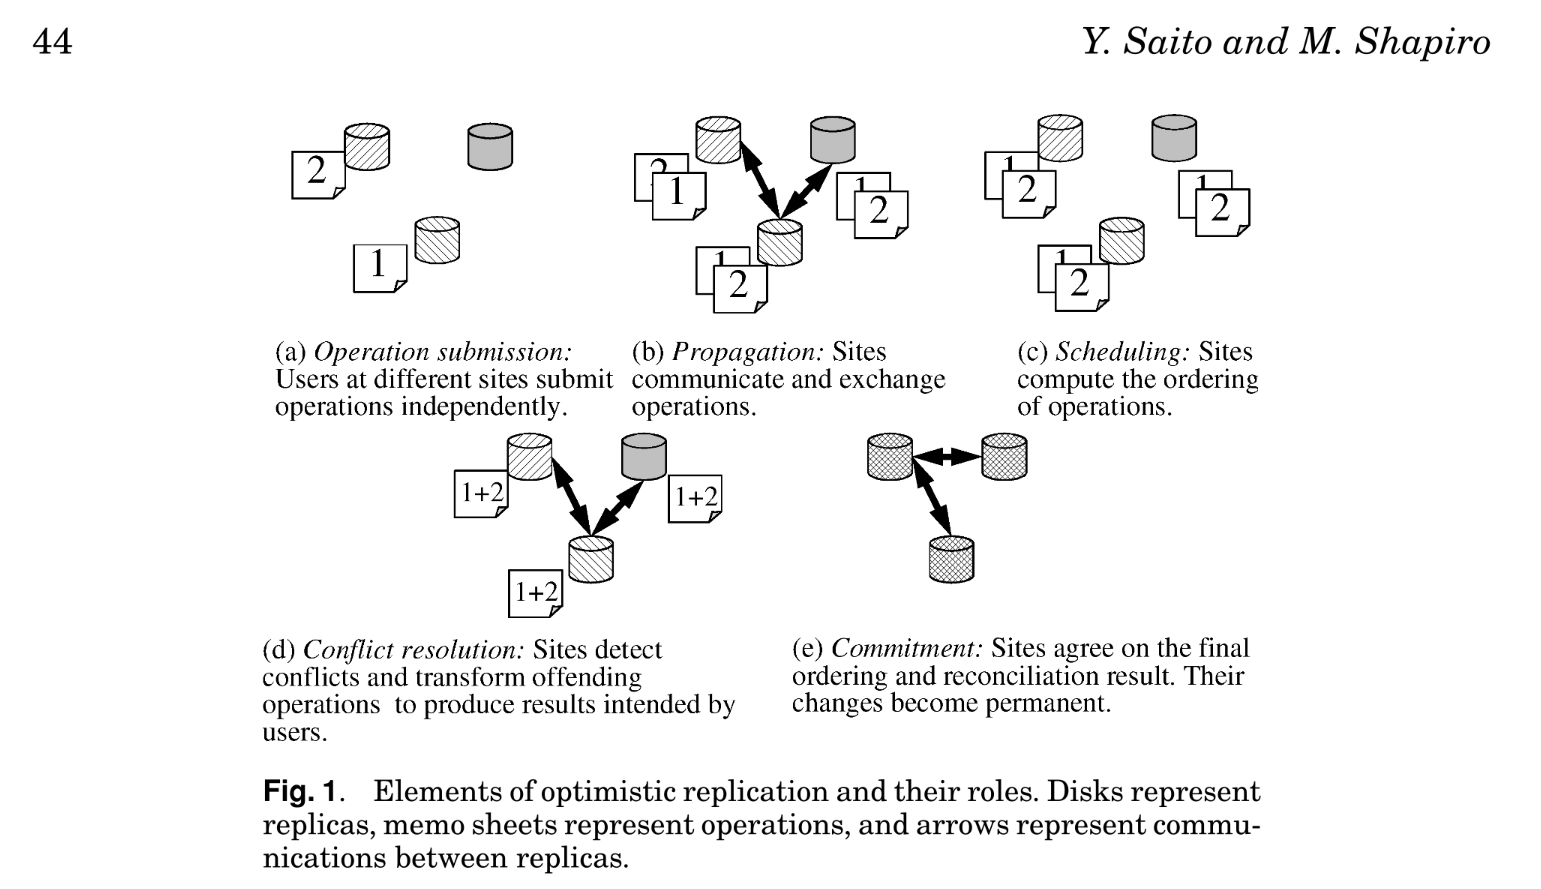
\includegraphics[width=1.25\linewidth,keepaspectratio]{../seminar5-replication/images/shapiro_saito_stages.png}
\end{center}

\end{frame}

%--------------------------------------------------
\section{История развития}

\begin{frame}
\frametitle{Операциональные преобразования (OT) - 1989}

\begin{columns}
\begin{column}{0.55\textwidth}

\medskip
\textbf{Ключевая идея:}
\begin{itemize}
  \item Операции отправляются как есть на все реплики
  \item При получении операция \emph{преобразуется} с учётом уже применённых операций
  \item Функция трансформации $T(op_1, op_2) \to op_1'$
\end{itemize}

\medskip
\textbf{Условие корректности (TP1):}\\
$op_1 \circ T(op_2, op_1) = op_2 \circ T(op_1, op_2)$

\medskip
\textbf{Системы:} Jupiter (Xerox PARC, 1995), Google Wave (2009), ShareJS, Atom Teletype.
\end{column}
\begin{column}{0.42\textwidth}
\begin{tikzpicture}[scale=0.85, every node/.style={font=\small}]
  \node[draw,rounded corners,fill=blue!15] (A0) at (0,3.5) {$S_0$};
  \node[draw,rounded corners,fill=blue!15] (B0) at (3,3.5) {$S_0$};

  \node[draw,rounded corners,fill=green!20] (A1) at (0,2.0) {$S_A$};
  \node[draw,rounded corners,fill=green!20] (B1) at (3,2.0) {$S_B$};

  \node[draw,rounded corners,fill=orange!20] (A2) at (0,0.5) {$S'$};
  \node[draw,rounded corners,fill=orange!20] (B2) at (3,0.5) {$S'$};

  \draw[->,thick] (A0) -- node[left]{$op_A$} (A1);
  \draw[->,thick] (B0) -- node[right]{$op_B$} (B1);

  \draw[->,dashed,blue] (A1) -- node[above,sloped,font=\tiny]{send $op_A$} (B1);
  \draw[->,dashed,red]  (B1) -- node[below,sloped,font=\tiny]{send $op_B$} (A1);

  \draw[->,thick] (A1) -- node[left,font=\tiny]{$T(op_B,op_A)$} (A2);
  \draw[->,thick] (B1) -- node[right,font=\tiny]{$T(op_A,op_B)$} (B2);
\end{tikzpicture}
\end{column}
\end{columns}

\end{frame}

\begin{frame}
\frametitle{Операциональные преобразования (OT) - 1989}

\vspace{0.3em}
\begin{alertblock}{Проблема OT}
В 2000-х возникла репутация о том, что OT-алгоритмы склонны быть некорректными.

При этом – активно используется в Google Docs до сих пор.
\end{alertblock}

\textbf{Online-демо}: {\bfseries \href{https://operational-transformation.github.io/}{operational-transformation.github.io}}

\end{frame}

\begin{frame}
\frametitle{Семантическая реконсиляция}

\begin{columns}
\begin{column}{0.60\textwidth}
\textbf{Marc Shapiro et al.\ (2000–2005), INRIA:}
\begin{itemize}
  \item Конфликты разрешаются \emph{семантически} — система знает смысл данных
  \item Reconciler — функция $R(s_1, s_2, s_\text{base})$ с учётом общего предка
  \item Позволяет более умные merge (diff3, operational semantics)
\end{itemize}

\bigskip
\textbf{Ограничения:}\\
Требует централизованного reconciler или 3-way merge; не масштабируется тривиально.
\end{column}
\begin{column}{0.37\textwidth}
\begin{tikzpicture}[scale=0.8, every node/.style={font=\small}]
  \node[draw,circle,fill=gray!20] (base) at (1.5,3) {base};
  \node[draw,circle,fill=blue!20] (s1) at (0,1.5) {$s_1$};
  \node[draw,circle,fill=red!20]  (s2) at (3,1.5) {$s_2$};
  \node[draw,circle,fill=green!30](res) at (1.5,0) {$s'$};

  \draw[->,thick] (base)--(s1) node[midway,left,font=\tiny]{edit A};
  \draw[->,thick] (base)--(s2) node[midway,right,font=\tiny]{edit B};
  \draw[->,thick,dashed] (s1)--(res);
  \draw[->,thick,dashed] (s2)--(res);
  \node[font=\tiny] at (1.5,0.55) {$R(s_1,s_2,\text{base})$};
\end{tikzpicture}
\end{column}
\end{columns}

\end{frame}

%--------------------------------------------------
\section{CRDT}

\begin{frame}
\frametitle{Мотивация и интуиция}

\begin{columns}
\begin{column}{0.52\textwidth}
\textbf{Почему CRDT?}
\begin{itemize}
  \item OT сложно реализовать корректно
  \item Семантическая реконсиляция требует координации
  \item Хотим: \textbf{локальные} операции + \textbf{гарантированная} сходимость
\end{itemize}

\bigskip
\textbf{Ключевая интуиция:}\\
Если структуры данных и операции спроектированы так, что результат \emph{не зависит от порядка и количества применений}, конфликтов не возникает в принципе.

\bigskip

\end{column}
\begin{column}{0.45\textwidth}
\begin{tikzpicture}[scale=0.78, every node/.style={font=\scriptsize}]
  % Three replicas
  \foreach \i/\col/\lbl in {0/blue!25/A, 1.8/red!25/B, 3.6/green!25/C}{
    \node[draw,minimum width=1.3cm,minimum height=0.7cm,fill=\col,rounded corners] 
      at (\i,2.8) {\textbf{Node \lbl}};
  }
  \node[font=\tiny] at (0,2.1)   {val=3};
  \node[font=\tiny] at (1.8,2.1) {val=5};
  \node[font=\tiny] at (3.6,2.1) {val=2};

  % Arrows for gossip
  \draw[->,bend left=20,dashed] (0.4,2.5) to (1.4,2.5);
  \draw[->,bend left=20,dashed] (2.2,2.5) to (3.2,2.5);
  \draw[->,bend right=30,dashed] (3.2,2.2) to (0.4,2.2);

  \node[draw,fill=yellow!30,rounded corners,minimum width=3.8cm] at (1.8,0.8) 
    {\textbf{merge: max per node}};
  \node at (1.8,0.2) {global = $3+5+2 = 10$};
  \draw[->,thick] (1.8,1.9) -- (1.8,1.2);
\end{tikzpicture}
\end{column}
\end{columns}

\end{frame}

\begin{frame}
\frametitle{Демо}
\begin{itemize}
    \item \href{https://www.iankduncan.com/engineering/2025-11-27-crdt-dictionary/}{The CRDT Dictionary: A Field Guide to Conflict-Free Replicated Data Types}
    \item \href{https://lars.hupel.info/topics/crdt/01-intro/}{An introduction to Conflict-Free Replicated Data Types}
\end{itemize}

\end{frame}

\begin{frame}
\frametitle{Определение CRDT и SEC}

\begin{definitionbox}[CRDT — Conflict-free Replicated Data Type (Shapiro et al., 2011)]
    \small
Реплицированный тип данных называется CRDT, если он реализует \textbf{сильную итоговую согласованность} (Strong Eventual Consistency, SEC).
\end{definitionbox}

\medskip
\begin{definitionbox}[SEC]
Реплицированный объект удовлетворяет SEC, если: \small
\begin{enumerate}
  \item \textbf{Eventual delivery:} каждое обновление, применённое на корректной реплике, в конечном счёте доставляется на все корректные реплики
  \item \textbf{Strong Convergence:} корректные реплики, получившие \emph{одинаковый набор} обновлений, находятся в \textbf{одинаковом состоянии}
\end{enumerate}
\end{definitionbox}

\medskip
\begin{alertblock}{SEC vs.\ EC (Eventual Consistency)}
    \small
EC гарантирует только eventual convergence «когда-нибудь»; SEC гарантирует convergence \emph{сразу при доставке одинакового набора обновлений} — это значительно сильнее.
\end{alertblock}

\end{frame}

\begin{frame}
\frametitle{Strong Eventual Consistency}

\begin{itemize}
  \item При доставке одного и того же набора обновлений все реплики гарантированно равны
  \item Порядок доставки не важен
  \item Обычно достигается через CRDT:
  \begin{itemize}
    \item операции \textbf{коммутативны}: $op_1 \circ op_2 = op_2 \circ op_1$
    \item merge \textbf{ассоциативен, коммутативен и идемпотентен}: $(s_1 \merge s_2) \merge s_3 = s_1 \merge (s_2 \merge s_3)$
  \end{itemize}
\end{itemize}

\begin{exampleblock}{Таксономия (Shapiro et al., 2011)}
\begin{center}
\begin{tikzpicture}[scale=0.85]
  \node[draw,fill=blue!20,rounded corners,minimum width=3cm] (crdt) at (0,0) {\textbf{CRDT}};
  \node[draw,fill=green!20,rounded corners] (cvr) at (-2,-1.3) {CvRDT};
  \node[draw,fill=orange!20,rounded corners] (cmr) at (2,-1.3) {CmRDT};
  \draw[->] (crdt) -- (cvr) node[midway,left,font=\tiny]{state-based};
  \draw[->] (crdt) -- (cmr) node[midway,right,font=\tiny]{op-based};
  \node[font=\scriptsize,align=center] at (-2,-2.1) {join-semilattice\\$\merge = \sqcup$};
  \node[font=\scriptsize,align=center] at (2,-2.1) {causal delivery\\commutative ops};
\end{tikzpicture}
\end{center}
\end{exampleblock}

\textbf{Примеры:} счетчики, множества, совместное редактирование документов.

\end{frame}

\begin{frame}
\frametitle{State-based vs.\ Operation-based CRDT}

\begin{columns}
\begin{column}{0.48\textwidth}
\begin{block}{CvRDT (State-based)}
\begin{itemize}
  \item Передаём \textbf{всё состояние} реплике
  \item Merge через $\sqcup$ (join / LUB)
  \item Требование: join-semilattice
  \item \textbf{+} простота: любой канал, идемпотентность
  \item \textbf{–} затраты на передачу состояния
\end{itemize}
\end{block}

\begin{tikzpicture}[scale=0.75,every node/.style={font=\scriptsize}]
  \node[draw,fill=blue!15,rounded corners] (r1) at (0,1) {$S_A$};
  \node[draw,fill=red!15,rounded corners]  (r2) at (3,1) {$S_B$};
  \draw[->,thick,blue] (r1) to[bend left=20] node[above]{full state $S_A$} (r2);
  \node[draw,fill=purple!20,rounded corners] (m) at (1.5,0) {$S_A \sqcup S_B$};
  \draw[->,thick] (r2) -- (m);
\end{tikzpicture}
\end{column}
\begin{column}{0.48\textwidth}
\begin{block}{CmRDT (Op-based)}
\begin{itemize}
  \item Передаём \textbf{операции}
  \item Операции должны быть \textbf{коммутативны}
  \item Требование: \emph{causal delivery} (FIFO или causal broadcast)
  \item \textbf{+} малый объём сообщений
  \item \textbf{–} надёжный канал с causal ordering
\end{itemize}
\end{block}

\begin{tikzpicture}[scale=0.75,every node/.style={font=\scriptsize}]
  \node[draw,fill=blue!15,rounded corners] (r1) at (0,1) {$S_A$};
  \node[draw,fill=red!15,rounded corners]  (r2) at (3,1) {$S_B$};
  \draw[->,thick,blue] (r1) to[bend left=20] node[above]{$op(a)$} (r2);
  \draw[->,thick,red]  (r2) to[bend left=20] node[below]{$op(b)$} (r1);
  \node[font=\tiny,align=center] at (1.5,0.1) {$op(a)\circ op(b) = op(b)\circ op(a)$};
\end{tikzpicture}
\end{column}
\end{columns}

\bigskip
\begin{exampleblock}{Эквивалентность}
Shapiro et al. (2011) доказали: CvRDT и CmRDT выразимы друг через друга при наличии соответствующих гарантий доставки.
\end{exampleblock}

\end{frame}

\begin{frame}
\frametitle{Определение CvRDT}

\begin{definitionbox}[Join-Semilattice / CvRDT]
$(S, \leq, \sqcup)$ — CvRDT, если:
\begin{itemize}
  \item $(S, \leq)$ — частично упорядоченное множество
  \item $\forall a,b \in S$: $a \sqcup b = \sup\{a,b\}$ (least upper bound)
  \item $\sqcup$ коммутативна, ассоциативна, идемпотентна
  \item Каждое обновление \textbf{монотонно}: $s \leq \text{update}(s)$
\end{itemize}
\end{definitionbox}

\begin{columns}
\begin{column}{0.48\textwidth}
\textbf{Диаграмма Хассе} для $\mathcal{P}(\{a,b,c\})$:
\begin{tikzpicture}[scale=0.75, every node/.style={font=\scriptsize}]
  \node (abc) at (1.5,3)  {$\{a,b,c\}$};
  \node (ab)  at (0,2)    {$\{a,b\}$};
  \node (ac)  at (1.5,2)  {$\{a,c\}$};
  \node (bc)  at (3,2)    {$\{b,c\}$};
  \node (a)   at (0,1)    {$\{a\}$};
  \node (b)   at (1.5,1)  {$\{b\}$};
  \node (c)   at (3,1)    {$\{c\}$};
  \node (emp) at (1.5,0)  {$\emptyset$};
  \draw (emp)--(a)--(ab)--(abc); \draw (emp)--(b)--(ab);
  \draw (b)--(bc)--(abc); \draw (emp)--(c)--(ac)--(abc);
  \draw (c)--(bc); \draw (a)--(ac);
\end{tikzpicture}
\end{column}
\begin{column}{0.48\textwidth}
\textbf{Свойство монотонности}:\\[0.3em]
Состояние реплики \emph{только растёт} по решётке. Это гарантирует сходимость: после любого merge результат $\geq$ обоих операндов.\\[0.6em]
\textbf{LUB явно:}
\[
  s_1 \sqcup s_2 \geq s_1,\; s_1 \sqcup s_2 \geq s_2
\]
\[
  \forall u: u\geq s_1 \land u\geq s_2 \Rightarrow u \geq s_1 \sqcup s_2
\]
\end{column}
\end{columns}

\end{frame}

\begin{frame}
\frametitle{Определение CmRDT}

\begin{definitionbox}[CmRDT — Op-based CRDT]
Реплицированный объект $(S, \mathit{do}, \mathit{apply})$ является CmRDT, если:
\begin{itemize}
  \item $\mathit{do}(op, s)$ выполняется \textbf{локально} и генерирует сообщение $m$
  \item $\mathit{apply}(m, s)$ применяется на удалённых репликах
  \item Параллельные операции \textbf{коммутативны}: $\mathit{apply}(m_1, \mathit{apply}(m_2,s)) = \mathit{apply}(m_2, \mathit{apply}(m_1,s))$
\end{itemize}
\end{definitionbox}

\begin{columns}
\begin{column}{0.55\textwidth}
\textbf{Условие коммутативности:}
\[
  m_1 \parallel m_2 \Rightarrow \mathit{apply}(m_1) \circ \mathit{apply}(m_2) = \mathit{apply}(m_2) \circ \mathit{apply}(m_1)
\]
Операции \emph{конкурентны} ($m_1 \parallel m_2$), если ни одна не зависит от другой в частичном порядке событий (Lamport, 1978).
\textbf{Доставка:} causal broadcast (например, по vector clock).
\end{column}
\begin{column}{0.42\textwidth}
\begin{tikzpicture}[scale=0.8, every node/.style={font=\scriptsize}]
  \node[draw,fill=blue!10] (a1) at (0,2.5) {$s$};
  \node[draw,fill=blue!10] (a2) at (0,1.5) {$s_A$};
  \node[draw,fill=blue!10] (a3) at (0,0.3) {$s'$};

  \node[draw,fill=red!10]  (b1) at (3,2.5) {$s$};
  \node[draw,fill=red!10]  (b2) at (3,1.5) {$s_B$};
  \node[draw,fill=red!10]  (b3) at (3,0.3) {$s'$};

  \draw[->,thick] (a1)--node[left]{$op_A$}(a2);
  \draw[->,thick] (b1)--node[right]{$op_B$}(b2);

  \draw[->,dashed,blue] (a2) to[bend left=15] node[above,font=\tiny]{$m_A$}(b2);
  \draw[->,dashed,red]  (b2) to[bend left=15] node[below,font=\tiny]{$m_B$}(a2);

  \draw[->,thick](a2)--node[left,font=\tiny]{$+m_B$}(a3);
  \draw[->,thick](b2)--node[right,font=\tiny]{$+m_A$}(b3);
  \node[font=\tiny] at (1.5,-0.1){$s' = s' \checkmark$};
\end{tikzpicture}
\end{column}
\end{columns}

\end{frame}

\begin{frame}
\frametitle{Зоопарк CRDT}

\begin{center}
\begin{tikzpicture}[
  scale=1.2,
  box/.style={draw,rounded corners,font=\scriptsize,align=center,minimum width=0.8cm,minimum height=0.6cm},
  every node/.style={font=\scriptsize}
]
  \node[box,fill=blue!20]   (crdt)  at (4,4.5) {\textbf{CRDT}};

  \node[box,fill=green!20]  (cnt)   at (0.5,3)   {Счётчики};
  \node[box,fill=orange!20] (reg)   at (3,3)     {Регистры};
  \node[box,fill=red!20]    (set)   at (5.5,3)   {Множества};
  \node[box,fill=purple!20] (seq)   at (7.5,3)   {Последо-\\вательности};

  \draw[->](crdt)--(cnt); \draw[->](crdt)--(reg);
  \draw[->](crdt)--(set); \draw[->](crdt)--(seq);

  \node[box,fill=green!10]  (gc)  at (-0.5,1.5) {G-Counter};
  \node[box,fill=green!10]  (pnc) at (1.5,1.5)  {PN-Counter};
  \draw[->](cnt)--(gc); \draw[->](cnt)--(pnc);

  \node[box,fill=orange!10] (lwr) at (2.2,1.5)  {LWW-Reg};
  \node[box,fill=orange!10] (mvr) at (3.8,1.5)  {MV-Reg};
  \draw[->](reg)--(lwr); \draw[->](reg)--(mvr);

  \node[box,fill=red!10]    (gs)  at (4.5,1.5)  {G-Set};
  \node[box,fill=red!10]    (2ps) at (5.8,1.5)  {2P-Set};
  \node[box,fill=red!10]    (ors) at (7.1,1.5)  {OR-Set};
  \draw[->](set)--(gs); \draw[->](set)--(2ps); \draw[->](set)--(ors);

  \node[box,fill=purple!10] (woot) at (6.5,0.3)  {WOOT};
  \node[box,fill=purple!10] (rga)  at (8.0,0.3)  {RGA};
  \node[box,fill=purple!10] (lgn)  at (7.2,-0.5) {Logoot/\\LSEQ};
  \draw[->](seq)--(woot); \draw[->](seq)--(rga); \draw[->](seq)--(lgn);
\end{tikzpicture}
\end{center}

\end{frame}

\begin{frame}
\frametitle{Отечественные исследователи}

\begin{columns}
\begin{column}{0.48\textwidth}
\textbf{Виктор Грищенко}\\
\begin{itemize}
  \item Автор \textbf{Chronofold} (2020) — CRDT для последовательностей на основе linked list с временными метками
  \item Концепция \textbf{Swarm} — децентрализованный объектная среда на основе CRDT
  \item Ранние работы по \textbf{RON} (Replicated Object Notation)
\end{itemize}
\end{column}
\begin{column}{0.48\textwidth}
\textbf{Юрий Сыровецкий}
\begin{itemize}
  \item Haskell-реализация CRDT (\texttt{crdts} на Hackage)
  \item Вклад в формализацию типов в функциональном стиле
\end{itemize}

\end{column}
\end{columns}


\end{frame}

%--------------------------------------------------
\section{Регистры}

\begin{frame}
\frametitle{Last-Writer-Wins Register (LWW-Register)}

\begin{columns}
\begin{column}{0.52\textwidth}
\textbf{Определение:}
\begin{itemize}
  \item Состояние: $(v, \ts)$ — значение и временная метка
  \item \texttt{write}$(v')$: $(\_, \_) \to (v', \mathit{now}())$
  \item \texttt{read}: возвращает $v$
  \item \texttt{merge}$((v_1,t_1),(v_2,t_2))$:
  \[
    = \begin{cases}(v_1,t_1) & \text{если } t_1 > t_2 \\ (v_2,t_2) & \text{иначе}\end{cases}
  \]
\end{itemize}

\medskip
\textbf{Метки:} Lamport clock, physical clock (NTP), hybrid logical clock (HLC).

\medskip
\textbf{Применяется:} Amazon DynamoDB (per-attribute LWW), Cassandra (по умолчанию).
\end{column}
\begin{column}{0.45\textwidth}
\begin{tikzpicture}[scale=0.8, every node/.style={font=\scriptsize}]
  \node[draw,fill=blue!15,rounded corners,align=center] (a) at (0,3) {Node A\\$(x, t=5)$};
  \node[draw,fill=red!15,rounded corners,align=center]  (b) at (3,3) {Node B\\$(y, t=3)$};
  \node[draw,fill=green!20,rounded corners](m) at (1.5,1.5) {merge};
  \node[draw,fill=green!30,rounded corners](r) at (1.5,0.3) {$(x, t=5)$ $\checkmark$};

  \draw[->,thick](a)--(m);
  \draw[->,thick](b)--(m);
  \draw[->,thick](m)--(r);
\end{tikzpicture}

\bigskip
\begin{alertblock}{Проблема LWW}
\small Записи могут теряться! Если $t_A \approx t_B$, один \texttt{write} «перекрывает» другой — семантика last-write-wins.
\end{alertblock}
\end{column}
\end{columns}

\end{frame}

\begin{frame}
\frametitle{Multi-Value Register (MVR)}

\begin{columns}
\begin{column}{0.52\textwidth}
\textbf{Идея:}\\
Вместо одного значения хранить \emph{множество} конкурентных значений.
Используем \textbf{vector clocks} для определения параллельности.

\medskip
\textbf{Состояние:} множество пар $\{(v_i, \mathbf{vc}_i)\}$

\medskip
\textbf{write}$(v)$ на реплике $i$:\\
— инкрементируем $\mathbf{vc}[i]$\\
— удаляем все записи, покрытые новым VC\\
— добавляем $(v, \mathbf{vc})$

\medskip
\textbf{merge}: объединяем множества, удаляем «dominated» записи.

\medskip
\textbf{read}: если $|\text{set}|>1$ — конфликт; приложение решает.

\medskip
\textbf{Пример:} Amazon S3 (siblings в Riak KV).
\end{column}
\begin{column}{0.45\textwidth}
\begin{tikzpicture}[scale=0.8, every node/.style={font=\scriptsize}]
  \node[draw,fill=blue!15,rounded corners,align=center] (a) at (0,3.2)
    {Node A\\write ``foo''\\vc=[1,0]};
  \node[draw,fill=red!15,rounded corners,align=center] (b) at (3,3.2)
    {Node B\\write ``bar''\\vc=[0,1]};
  \node[draw,fill=orange!20,rounded corners,align=center] (m) at (1.5,1.5)
    {merge →\\$\{(\texttt{foo},[1,0]),(\texttt{bar},[0,1])\}$};
  \node[font=\tiny,align=center] at (1.5,0.5)
    {Concurrent writes!\\Application picks or shows both.};
  \draw[->,thick](a)--(m);
  \draw[->,thick](b)--(m);
\end{tikzpicture}
\end{column}
\end{columns}

\end{frame}

%--------------------------------------------------
\section{Множества}

\begin{frame}
\frametitle{Grow-only Set (G-Set)}

\textbf{Простейший CRDT:} элементы только добавляются, никогда не удаляются.

\begin{columns}
\begin{column}{0.45\textwidth}
\textbf{Формально:}
\begin{itemize}
  \item Состояние: $S \subseteq \mathcal{U}$
  \item \texttt{add}$(e)$: $S \leftarrow S \cup \{e\}$
  \item \texttt{lookup}$(e)$: $e \in S$
  \item \texttt{merge}$(S_1, S_2) = S_1 \cup S_2$
\end{itemize}

\medskip
Решётка: $(\mathcal{P}(\mathcal{U}), \subseteq, \cup)$

\medskip
\textbf{Свойства:}\\
$S_1 \cup S_2$ — LUB в решётке подмножеств. Монотонность: $S \subseteq S \cup \{e\}$. Все аксиомы CvRDT выполнены тривиально.
\end{column}
\begin{column}{0.52\textwidth}
\begin{tikzpicture}[scale=0.80, every node/.style={font=\scriptsize}]
  \node[draw,fill=blue!15,rounded corners,align=center] (a) at (0,2.5)
    {A: $\{1,2,3\}$};
  \node[draw,fill=red!15,rounded corners,align=center]  (b) at (3.5,2.5)
    {B: $\{2,4,5\}$};
  \node[draw,fill=green!25,rounded corners] (m) at (1.75,1.1)
    {merge: $\{1,2,3,4,5\}$};
  \draw[->,thick](a)--(m);
  \draw[->,thick](b)--(m);

  \draw[->,dashed,blue](a) to[bend left=20] node[above,font=\tiny]{sync} (b);
  \draw[->,dashed,red](b) to[bend left=20] node[below,font=\tiny]{sync} (a);
\end{tikzpicture}

\vspace{0.2em}
\begin{exampleblock}{Применение}
\small Набор тегов, список увиденных событий, распределённый blacklist, membership views.
\end{exampleblock}
\end{column}
\end{columns}

\end{frame}

\begin{frame}
\frametitle{Two-Phase Set (2P-Set)}

\textbf{Идея:} разрешить \emph{удаление}, но только \textbf{один раз} (deleted $\rightarrow$ нельзя добавить снова).

\begin{columns}
\begin{column}{0.50\textwidth}
\textbf{Состояние:} два G-Set: $A$ (добавленные), $R$ (удалённые), $R \subseteq A$

\[
  \texttt{lookup}(e) \Leftrightarrow e \in A \setminus R
\]

\begin{itemize}
  \item \texttt{add}$(e)$: $A \leftarrow A \cup \{e\}$
  \item \texttt{remove}$(e)$: \textbf{только если} $e \in A$: $R \leftarrow R \cup \{e\}$
  \item \texttt{merge}: $\langle A_1 \cup A_2,\; R_1 \cup R_2 \rangle$
\end{itemize}

\medskip
\textbf{Ограничение:} при конкурентных \texttt{add} и \texttt{remove} — побеждает \texttt{remove} (remove-wins bias) по умолчанию.
\end{column}
\begin{column}{0.47\textwidth}
\begin{tikzpicture}[scale=0.78, every node/.style={font=\scriptsize}]
  \node[draw,fill=blue!15,rounded corners,align=center] at (0,3)
    {A: $A=\{a,b\}$\\$R=\{b\}$};
  \node[draw,fill=red!15,rounded corners,align=center] at (3,3)
    {B: $A=\{a,c\}$\\$R=\emptyset$};
  \node[draw,fill=green!20,rounded corners,align=center] at (1.5,1.5)
    {merge:\\$A=\{a,b,c\}$\\$R=\{b\}$\\visible: $\{a,c\}$};
  \draw[->,thick](0,2.65)--(1.5,2.0);
  \draw[->,thick](3,2.65)--(1.5,2.0);
\end{tikzpicture}
\end{column}
\end{columns}

\end{frame}

\begin{frame}
\frametitle{Observed-Remove Set (OR-Set)}

\begin{columns}
\begin{column}{0.52\textwidth}
\textbf{Проблема 2P-Set:} нельзя повторно добавить удалённый элемент.\\[0.3em]
\textbf{OR-Set решает это} с помощью уникальных тегов (Shapiro et al., 2011).

\medskip
\textbf{Состояние:} $\{(e, \text{uid})\}$ — мультимножество пар

\begin{itemize}
  \item \texttt{add}$(e)$: добавляем $(e, \text{uid}_\text{fresh})$
  \item \texttt{remove}$(e)$: удаляем все пары $(e, \_)$ \emph{которые наблюдала текущая реплика}
  \item \texttt{lookup}$(e)$: $\exists$ пара $(e, \_)$ в состоянии
  \item \texttt{merge}: объединение множеств пар
\end{itemize}

\medskip
\textbf{Семантика:} \textbf{add-wins}! Параллельный \texttt{add} побеждает \texttt{remove}.

\end{column}
\begin{column}{0.45\textwidth}
\begin{tikzpicture}[scale=0.78, every node/.style={font=\scriptsize}]
  \node[draw,fill=blue!15,rounded corners,align=center] (a0) at (0,4)
    {A: $\{(x,u_1)\}$};
  \node[draw,fill=red!15,rounded corners,align=center]  (b0) at (3.5,4)
    {B: $\{(x,u_1)\}$};

  \node[draw,fill=blue!25,rounded corners,align=center] (a1) at (0,2.5)
    {A: add $x$ again\\$\{(x,u_1),(x,u_2)\}$};
  \node[draw,fill=red!25,rounded corners,align=center]  (b1) at (3.5,2.5)
    {B: remove $x$\\$\{\ \}$};

  \node[draw,fill=green!20,rounded corners,align=center](m) at (1.75,1.0)
    {merge: $\{(x,u_2)\}$\\$x$ visible};

  \draw[->,thick](a0)--(a1); \draw[->,thick](b0)--(b1);
  \draw[->,thick](a1)--(m); \draw[->,thick](b1)--(m);
  \node[font=\tiny,align=center] at (1.75,0.2){add-wins: $u_2$ не был виден B};
\end{tikzpicture}
\end{column}
\end{columns}

\end{frame}

\begin{frame}
\frametitle{Positive-Negative Set и Unique Set}

\begin{columns}
\begin{column}{0.48\textwidth}
\begin{block}{PN-Set (Positive-Negative)}
\begin{itemize}
  \item Два G-Set: $P$ (добавления), $N$ (удаления)
  \item \texttt{lookup}$(e)$: $|P_e| > |N_e|$ (считаем вхождения)
  \item Позволяет повторное добавление после удаления
  \item Проблема: \texttt{remove} без предварительного \texttt{add} — некорректно
\end{itemize}
\end{block}
\end{column}
\begin{column}{0.48\textwidth}
\begin{block}{U-Set (Unique Set)}
\begin{itemize}
  \item Каждый элемент имеет \textbf{уникальный идентификатор}
  \item add$(e,\text{uid})$: добавить $(e,\text{uid})$
  \item remove$(e,\text{uid})$: удалить $(e,\text{uid})$
  \item Гарантирует: одна \texttt{add} → один \texttt{remove}
  \item Реализация: часто через OR-Set с UUID
\end{itemize}
\end{block}
\end{column}
\end{columns}

\end{frame}

\begin{frame}
\frametitle{Сравнение}

\begin{exampleblock}{Сравнительная таблица множеств}
\small
\begin{tabular}{lcccc}
\toprule
\textbf{Тип} & \textbf{Удал.} & \textbf{Повтор. add} & \textbf{Conc. bias} & \textbf{Сложность} \\
\midrule
G-Set   & нет  & н/д    & —           & $O(n)$ \\
2P-Set  & да   & нет    & remove-wins & $O(n)$ \\
OR-Set  & да   & да     & add-wins    & $O(n^2)$ \\
PN-Set  & да   & да     & зависит     & $O(n)$ \\
\bottomrule
\end{tabular}
\end{exampleblock}

\end{frame}

%--------------------------------------------------
\section{Счётчики}

\begin{frame}
\frametitle{Grow-only Counter (G-Counter)}

\begin{columns}
\begin{column}{0.52\textwidth}
\textbf{Состояние:} вектор $\mathbf{v} \in \mathbb{N}^n$ (по одному счётчику на узел)

\[
  \texttt{value}() = \sum_{i=1}^{n} \mathbf{v}[i]
\]

\begin{itemize}
  \item \texttt{increment()} на узле $i$: $\mathbf{v}[i] \mathrel{+}= 1$
  \item \texttt{merge}$(\mathbf{v}_A, \mathbf{v}_B)[i] = \max(\mathbf{v}_A[i], \mathbf{v}_B[i])$
\end{itemize}

\medskip
\textbf{Решётка:} $(\mathbb{N}^n, \leq_\text{comp}, \max)$\\
Где $\mathbf{u} \leq \mathbf{v} \Leftrightarrow \forall i: u_i \leq v_i$

\medskip
\textbf{Применение:} счётчик лайков, просмотров, голосов.

\medskip
\textbf{Гарантия:} никаких потерь инкрементов, любой порядок merge даёт одинаковый результат.
\end{column}
\begin{column}{0.45\textwidth}
\begin{tikzpicture}[scale=0.82, every node/.style={font=\scriptsize}]
  % Initial state
  \node[font=\footnotesize,align=center] at (1.5,4.2) {\textbf{3 узла, начало: [0,0,0]}};

  \node[draw,fill=blue!15,rounded corners,align=center] at (0,3.0)
    {A: [2,0,0]};
  \node[draw,fill=red!15,rounded corners,align=center]  at (1.8,3.0)
    {B: [0,3,0]};
  \node[draw,fill=green!15,rounded corners,align=center]at (3.6,3.0)
    {C: [0,0,1]};

  \node[draw,fill=purple!15,rounded corners,align=center] at (1.8,1.8)
    {merge all:\\$[\max(2,0,0),\max(0,3,0),\max(0,0,1)]$\\$=[2,3,1]$};

  \node[draw,fill=yellow!30,rounded corners] at (1.8,0.6)
    {value $= 2+3+1 = 6$};

  \draw[->,thick](0.7,2.7)--(1.8,2.3);
  \draw[->,thick](1.8,2.7)--(1.8,2.3);
  \draw[->,thick](2.9,2.7)--(1.8,2.3);
  \draw[->,thick](1.8,1.4)--(1.8,0.9);
\end{tikzpicture}
\end{column}
\end{columns}

\end{frame}

\begin{frame}
\frametitle{Positive-Negative Counter (PN-Counter)}

\textbf{Идея:} объединить два G-Counter — $P$ для increment, $N$ для decrement.

\[
  \textbf{value}() = \sum_i P[i] - \sum_i N[i]
\]

\begin{columns}
\begin{column}{0.50\textwidth}
\begin{itemize}
  \item \texttt{increment()} на узле $i$: $P[i] \mathrel{+}= 1$
  \item \texttt{decrement()} на узле $i$: $N[i] \mathrel{+}= 1$
  \item \texttt{merge}: $\max$ покоординатно для $P$ и $N$
\end{itemize}

\medskip
\textbf{Ограничение:} значение может быть отрицательным, но отдельные компоненты $P$, $N$ только растут.

\medskip
\textbf{Применение:} reddit score (upvotes - downvotes), баланс игровой валюты.

\medskip
\textbf{Масштабирование:} $O(n)$ память при $n$ узлах. Для больших систем используют delta-CRDT.
\end{column}
\begin{column}{0.47\textwidth}
\begin{tikzpicture}[scale=0.8, every node/.style={font=\scriptsize}]
  \node[draw,fill=blue!15,rounded corners,align=center] at (0,3.0)
    {A:\\$P=[3,0], N=[1,0]$\\val=$3-1=2$};
  \node[draw,fill=red!15,rounded corners,align=center] at (3.2,3.0)
    {B:\\$P=[0,2], N=[0,2]$\\val=$2-2=0$};
  \node[draw,fill=green!20,rounded corners,align=center] at (1.6,1.4)
    {merge:\\$P=[3,2], N=[1,2]$\\val $=5-3=2$};
  \draw[->,thick](0.8,2.6)--(1.6,2.0);
  \draw[->,thick](2.4,2.6)--(1.6,2.0);
\end{tikzpicture}
\end{column}
\end{columns}

\end{frame}

%--------------------------------------------------
\section{Другие структуры данных}

\begin{frame}
\frametitle{Add-only Monotonic DAG}

\textbf{CRDT-граф:} добавление вершин и рёбер, без удаления. Реализуется как два G-Set: $V$ (вершины), $E$ (рёбра).

\medskip
\textbf{Свойство монотонности DAG:} при добавлении ребра $(u,v)$ — предикат проверяется \emph{локально}; merge может нарушить DAG-условие (отсутствие циклов), поэтому часто используют \textbf{только partial order} как инвариант.

\begin{center}
\begin{tikzpicture}[scale=0.85, every node/.style={font=\scriptsize},
  node/.style={draw,circle,fill=blue!20,minimum size=0.55cm}]
  \node[node] (a) at (0,1.5) {a};
  \node[node] (b) at (1.5,1.5) {b};
  \node[node] (c) at (3,1.5) {c};
  \node[node] (d) at (1.5,0) {d};
  \draw[->,thick](a)--(b); \draw[->,thick](b)--(c);
  \draw[->,thick](a)--(d); \draw[->,thick](d)--(c);

  \node[font=\tiny,align=left] at (5.5,0.9)
    {Replica 1:\\add edge $(b,d)$};
  \node[font=\tiny,align=left] at (5.5,0.3)
    {Replica 2:\\add vertex $e$, add edge $(c,e)$};

  \node[node,fill=orange!20] (e) at (4.5,1.5) {e};
  \draw[->,thick,dashed,orange](c)--(e);
  \draw[->,thick,dashed,blue](b) to[bend right=20] (d);
\end{tikzpicture}
\end{center}

\textbf{Применение:} системы контроля версий (commit graph), workflow engines, causality tracking.

\end{frame}

\begin{frame}
\frametitle{Causal Tree и 2P-Set Graph}

\begin{columns}
\begin{column}{0.48\textwidth}
\begin{block}{Causal Tree (CT)}
\begin{itemize}
  \item Каждая операция — узел дерева с ссылкой на \textbf{причину} (parent op)
  \item Структура: $\{(id, \text{parent\_id}, \text{payload})\}$
  \item Базис для WOOT, RGA, Treedoc
  \item Tombstone: удалённые узлы маркируются, но не удаляются
  \item Исп. в Atom Teletype, xi-editor
\end{itemize}
\end{block}
\end{column}
\begin{column}{0.48\textwidth}
\begin{block}{2P-Set Graph}
\begin{itemize}
  \item Два 2P-Set: $V$ (вершины), $E$ (рёбра)
  \item \texttt{addVertex}, \texttt{addEdge}, \texttt{removeVertex}, \texttt{removeEdge}
  \item Инвариант: $e=(u,v) \in E \Rightarrow u \in V \land v \in V$
  \item Поддержание инварианта при merge — сложность
  \item Shapiro et al. (2011) предлагают \textbf{vertex-removal precondition}
\end{itemize}
\end{block}
\end{column}
\end{columns}

\end{frame}

%--------------------------------------------------
% \section{Последовательности (Sequence CRDT)}

% \begin{frame}
% \frametitle{WOOT (Without Operational Transformation)}

% \textit{Oster et al., CSCW 2006}

% \begin{columns}
% \begin{column}{0.52\textwidth}
% \textbf{Каждый символ:} $\langle id, v, W_L, W_R, \text{visible}\rangle$
% \begin{itemize}
%   \item $id$ — уникальный идентификатор (сайт, clock)
%   \item $W_L$, $W_R$ — соседи \emph{в момент вставки}
%   \item При merge: вставляем символ, используя $W_L$, $W_R$ для определения позиции
%   \item Конкурентные вставки в одну позицию разрешаются детерминированным tiebreaking по $id$
% \end{itemize}
% \textbf{Сложность:} $O(n^2)$ на вставку в худшем случае (много конкурентных вставок).
% \end{column}
% \begin{column}{0.45\textwidth}
% \begin{tikzpicture}[scale=0.80, every node/.style={font=\scriptsize}]
%   % Document sequence
%   \node[font=\small] at (1.5, 3.2) {Документ: \texttt{[B·E·G·I·N]}};
%   \foreach \c/\x in {B/0, E/0.7, G/1.4, I/2.1, N/2.8}{
%     \node[draw,minimum size=0.5cm,fill=blue!15] at (\x,2.5) {\c};
%   }
%   % Insert H between G and I
%   \draw[->,red,thick] (1.4,2.0) -- (1.75,2.25);
%   \node[draw,minimum size=0.5cm,fill=red!25] at (1.75,1.5) {H};
%   \node[font=\tiny,red,align=center] at (1.75,1.0) {insert H\\between G,I};
%   \node[font=\tiny,align=center] at (1.5,0.3)
%     {Result: B·E·G·H·I·N};
% \end{tikzpicture}
% \end{column}
% \end{columns}

% \end{frame}

% \begin{frame}
% \frametitle{RGA (Replicated Growable Array)}

% \textit{Roh et al., Journal of Parallel and Distributed Computing, 2011}

% \begin{columns}
% \begin{column}{0.52\textwidth}
% \textbf{Идея:} связный список с уникальными s4vector $(s, sum, sid, seq)$
% \begin{itemize}
%   \item Каждый элемент: $\langle s4, v, \text{next}, \text{deleted}\rangle$
%   \item Вставка: находим predecessor по s4, вставляем после него
%   \item При конфликте (два insert после одного и того же): сортировка по s4 (timestamp desc)
%   \item Tombstone для удалений (элемент остаётся в списке, маркируется)
% \end{itemize}

% \medskip
% \textbf{Сложность:} $O(n)$ для вставки, $O(1)$ амортизированного для конвергентных вставок.

% \medskip
% \textbf{Применения:} Riak DT, Automerge (ранняя версия), Yjs (частично).
% \end{column}
% \begin{column}{0.45\textwidth}
% \begin{tikzpicture}[scale=0.75, every node/.style={font=\tiny},
%   elem/.style={draw,rounded corners,fill=blue!15,minimum width=0.9cm,minimum height=0.5cm}]

%   \node[elem] (s) at (0,3.5) {\textsc{head}};
%   \node[elem] (a) at (1.1,3.5) {H\\$t=1$};
%   \node[elem] (b) at (2.2,3.5) {e\\$t=2$};
%   \node[elem] (c) at (3.3,3.5) {y\\$t=3$};
%   \draw[->,thick](s)--(a)--(b)--(c);

%   % Concurrent inserts after 'e'
%   \node[elem,fill=red!20]  (x) at (2.2,2.3) {l\\$t=4_A$};
%   \node[elem,fill=green!20](y) at (3.4,2.3) {l\\$t=4_B$};
%   \draw[->,dashed,red](b)--(x);
%   \draw[->,dashed,green](b)--(y);

%   \node[font=\tiny,align=center] at (2,1.3)
%     {sort by timestamp desc:\\$t=4_B > t=4_A$ (by site)\\Result: H·e·$l_B$·$l_A$·y};
% \end{tikzpicture}
% \end{column}
% \end{columns}

% \end{frame}

% \begin{frame}
% \frametitle{Logoot и LSEQ}

% \textit{Weiss et al., ICDCS 2009 (Logoot); Nedelec et al., DocEng 2013 (LSEQ)}

% \begin{columns}
% \begin{column}{0.52\textwidth}
% \textbf{Logoot:} каждому элементу присваивается \textbf{уникальный позиционный идентификатор} из упорядоченного пространства $\mathcal{I}$.
% \begin{itemize}
%   \item $id = [(p_1, s_1), (p_2, s_2), \ldots]$ — список пар (позиция, сайт)
%   \item Вставка между $id_L$ и $id_R$: выбрать $id$ с $id_L < id < id_R$
%   \item Документ = упорядоченное множество $(id, v)$ пар
%   \item Удаление: просто удалить по $id$
% \end{itemize}

% \medskip
% \textbf{LSEQ:} адаптивное выделение идентификаторов для контроля длины пути — решает проблему «надувания» id в Logoot.
% \end{column}
% \begin{column}{0.45\textwidth}
% \begin{tikzpicture}[scale=0.75, every node/.style={font=\scriptsize}]
%   \node at (1.5,3.8) {\textbf{Идентификаторный интервал}};
%   \draw[thick,->] (0,3) -- (3.2,3) node[right] {$\mathcal{I}$};
%   \node[below] at (0,3) {$-\infty$};
%   \node[below] at (3,3) {$+\infty$};

%   \node[draw,circle,fill=blue!25,inner sep=1pt] (a) at (0.8,3) {};
%   \node[draw,circle,fill=blue!25,inner sep=1pt] (b) at (2.4,3) {};
%   \node[below,font=\tiny] at (0.8,2.9) {$id_L$};
%   \node[below,font=\tiny] at (2.4,2.9) {$id_R$};

%   \node[draw,circle,fill=red!40,inner sep=1pt] (c) at (1.6,3) {};
%   \node[above,font=\tiny,red] at (1.6,3.05) {new $id$};

%   \draw[<->,thick,blue] (0.8,2.4) -- (2.4,2.4) node[midway,below,font=\tiny]{free space};

%   \node[font=\tiny,align=center] at (1.5,1.8)
%     {LSEQ: адаптивно\\ чередует стратегии\\boundary+ / boundary-\\для balance дерева};
% \end{tikzpicture}
% \end{column}
% \end{columns}

% \end{frame}

% \begin{frame}
% \frametitle{Treedoc}

% \textit{Preguiça et al., IPDPS 2009}

% \begin{columns}
% \begin{column}{0.52\textwidth}
% \textbf{Идея:} последовательность как бинарное дерево с \emph{in-order traversal}.

% \begin{itemize}
%   \item Узел дерева = элемент + уникальный $id$ (путь в дереве)
%   \item Идентификатор пути естественно упорядочен: in-order traversal
%   \item Вставка между $L$ и $R$: добавить узел как левый потомок следующего или правый потомок текущего
%   \item \textbf{Disambiguator} (site id) для конкурентных вставок в один узел (mini-tree)
% \end{itemize}

% \medskip
% \textbf{Компакция:} tombstone-узлы без потомков удаляются при synchronization — уникальность CRDT!

% \end{column}
% \begin{column}{0.45\textwidth}
% \begin{tikzpicture}[scale=0.78, every node/.style={font=\scriptsize},
%   nd/.style={draw,circle,fill=blue!20,minimum size=0.55cm}]
%   \node[nd] (r) at (2,3.5) {m};
%   \node[nd] (l) at (0.8,2.4) {a};
%   \node[nd] (rr) at (3.2,2.4) {z};
%   \node[nd] (lr) at (1.6,1.3) {n};
%   \draw[-,thick](r)--(l); \draw[-,thick](r)--(rr);
%   \draw[-,thick](l)--(lr);

%   \node[font=\tiny,align=center] at (2,0.5)
%     {in-order: a, m, n, z\\(document order)};
%   \node[nd,fill=red!20] (ins) at (2.5,1.3) {o};
%   \draw[-,thick,dashed,red](rr)--(ins);
%   \node[font=\tiny,red,align=center] at (3.5,0.5) {insert 'o'\\after 'n'};
% \end{tikzpicture}
% \end{column}
% \end{columns}

% \end{frame}

% \begin{frame}
% \frametitle{Chronofold}

% \textit{Victor Grishchenko, arXiv:2002.09511, 2020}

% \begin{columns}
% \begin{column}{0.55\textwidth}
% \textbf{Ключевые идеи:}
% \begin{itemize}
%   \item Хранить операции в \textbf{chrono-order} (timestamp), не в document order
%   \item \textbf{Implicit linked list:} поддерживается массив «следующих» указателей $\mathit{nxt}[\cdot]$
%   \item Document order восстанавливается обходом implicit list за $O(n)$
%   \item Вставка новой операции: $O(1)$ амортизированно при FIFO доставке
% \end{itemize}

% \medskip
% \textbf{Формально:}\\
% $\text{CF} = (A, \mathit{nxt}, \mathit{ref})$ где:
% \begin{itemize}
%   \item $A[t]$ — операция с таймером $t$
%   \item $\mathit{ref}[t]$ — $t$ ссылается на предыдущую операцию
%   \item $\mathit{nxt}[t]$ — implicitly maintained sibling list
% \end{itemize}

% \end{column}
% \begin{column}{0.42\textwidth}
% \begin{tikzpicture}[scale=0.78, every node/.style={font=\scriptsize}]
%   \node[font=\small] at (1.5,4) {\textbf{Chrono order} (массив)};
%   \foreach \t/\c/\x in {1/H/0, 2/e/0.8, 3/l/1.6, 4/p/2.4, 5/!/3.2}{
%     \node[draw,fill=blue!15,minimum size=0.55cm] at (\x,3.2) {\c};
%     \node[font=\tiny] at (\x, 3.6) {$t=\t$};
%   }
%   % nxt pointers (document order via linked list)
%   % Suppose insert 'l2' at t=6 after t=2 (ref=e)
%   \node[draw,fill=red!20,minimum size=0.55cm] at (0,2.0) {l};
%   \node[font=\tiny,red] at (0,1.55) {$t=6$, ref=2};
%   \draw[->,red,thick,bend right=20] (0,1.8) to node[left,font=\tiny]{nxt} (0.8,3.0);
%   \node[font=\tiny,align=center] at (1.8,1.0)
%     {Document order:\\H·e·l·l·p·!\\(follow nxt links)};
% \end{tikzpicture}
% \end{column}
% \end{columns}

% \end{frame}

% \begin{frame}
% \frametitle{Fugue и FugueMax}

% \textit{Weidner, Nicholas, Rand, arXiv:2305.00583, 2023}

% \begin{columns}
% \begin{column}{0.55\textwidth}
% \textbf{Мотивация:}\\
% Существующие CRDT для последовательностей (RGA, YATA, Logoot) не имеют \textbf{формальных гарантий качества порядка} при конкурентных вставках. Вводится понятие \textbf{non-interleaving}.

% \medskip
% \begin{definitionbox}[Non-interleaving]
% \small Пусть пользователи A и B конкурентно вставляют последовательности символов $a_1\ldots a_k$ и $b_1\ldots b_m$ в одну позицию. CRDT \emph{не перемежает} их, если итоговый порядок — либо $a_1\ldots a_k b_1\ldots b_m$, либо $b_1\ldots b_m a_1\ldots a_k$.
% \end{definitionbox}

% \medskip
% \textbf{Результат:} RGA, Logoot, LSEQ — \emph{нарушают} non-interleaving. Fugue — \textbf{гарантирует}.

% \end{column}
% \begin{column}{0.42\textwidth}
% \textbf{FugueMax:}\\
% Расширение с явным понятием «maximal non-interleaving» — оптимально для UX.

% \medskip
% \begin{tikzpicture}[scale=0.80, every node/.style={font=\scriptsize}]
%   \node[font=\footnotesize,align=center] at (1.5,3.2) {Конкурентная вставка};
%   \node[draw,fill=blue!15,rounded corners,align=center] at (0.7,2.3)
%     {A вставляет\\``foo''};
%   \node[draw,fill=red!15,rounded corners,align=center] at (2.5,2.3)
%     {B вставляет\\``bar''};
%   \node[draw,fill=green!20,rounded corners,align=center] at (1.5,1.1)
%     {Fugue:\\``foobar'' или ``barfoo''\\(не ``fbaoor'')};
%   \draw[->,thick](0.7,2.0)--(1.5,1.5);
%   \draw[->,thick](2.5,2.0)--(1.5,1.5);

%   \node[draw,fill=orange!20,rounded corners,align=center] at (1.5,0.1)
%     {RGA может дать:\\``fboaor'' ← плохо!};
% \end{tikzpicture}
% \end{column}
% \end{columns}

% \end{frame}

%--------------------------------------------------
\begin{frame}
\frametitle{Открытые проблемы}

\begin{exampleblock}{Открытые вопросы}
\small
\begin{itemize}
  \item Delta-CRDT (меньше трафика, Almeida et al., 2018)
  \item Pure op-based CRDT (Baquero et al., 2017)
  \item CRDT в БД: Electric SQL, Ditto, Automerge 2.0
\end{itemize}
\end{exampleblock}

\end{frame}

\section{Итоги}

\begin{frame}
\frametitle{Итоги}

\begin{itemize}
\item Нового домашнего задания 3 пока нет.
\end{itemize}


\end{frame}

\end{document}